\subsection{实验目的}
对于给定的遥感任务,根据本专业的专业基础课以及专业课知识,借鉴本课程前期所进行的一些实验中的原理、流程以及实验方法,自主设计给定任务的解决方案与实验方法及流程,完成实验结果的分析。
\subsection{实验原理}
\subsubsection{新型差异图像的构造方法}
在SAR图像差异图的构造中,差值法和比值法 是最常用的两种方法。图像差值法是通过对两幅同 一地区不同时刻的 SAR 图像直接逐像素相减,从而得到差异影像图。设X1与X2分别表示为同一地区 在不同时刻获取的两幅SAR图像,图像大小为
$H\times W$,则图像差值法的计算方法如下式所示:
\begin{equation}
X_d(i, j) = \abs{X_1(i, j) - X_2(i, j)}
\end{equation}
将图像的对数比法和均值比法如下式所示
\begin{eqnarray}
Xd_2(i, j) = X_1(i, j)/X_2(i, j) \\
Xd_3(i, j) = 255\times\abs{\ln(X_1(i, j)/X_2(i, j))} \\
Xd_4(i, j) = 255\times\left( 1-\min\left(\frac{\mu_1(i, j)}{\mu_2(i, j)}, \frac{\mu_2(i, j)}{\mu_1(i, j)}\right) \right)
\end{eqnarray}
所以新的差异图像构造方法为
\begin{equation}
Xd(i, j) = \frac{255\times(\ln(\mu_a(i, j) + 1) - \ln(\mu_b(i, j) + 1))}{\max(Xd) - \min(Xd)}
\end{equation}
其中,$\mu_a$表示的是两幅图像中灰度值总和较大的图像中以坐标(i,j)为中心的3x3邻域 窗口内像素的灰度均值,$\mu_b$表示的是两幅图像中灰度值总和较小的图像中以坐标(i,j)为中心的3x3邻域 窗口内像素的灰度均值。
\subsection{实验流程}
\begin{figure}[H]
	\centering
	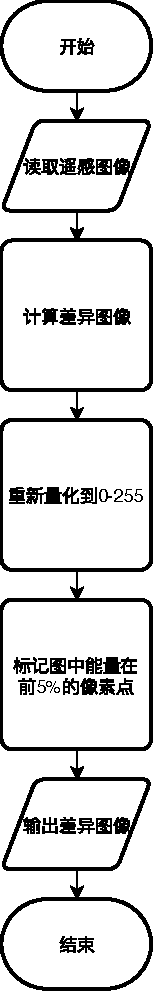
\includegraphics[width=0.15\linewidth]{figure/FinalFlowchart.pdf}
	\caption{实验过程流程图}
\end{figure}
\subsection{实验程序}
\lstinputlisting[caption={图像差异检测程序}]{"../Executable Script/Exp 14/main.m"}
\lstinputlisting[caption={新型差异图像检测函数FusionDifferDetection}]{"../Function Library/FusionDifferDetection.m"}
\lstinputlisting[caption={自动重新量化灰度值函数AutoGrayScale}]{"../Function Library/AutoGrayScale.m"}
\lstinputlisting[caption={自动二值化图像函数AutoBinarizeImage}]{"../Function Library/AutoBinarizeImage.m"}
\lstinputlisting[caption={虚警率计算函数ClassificationFalseAlarmRate}]{"../Function Library/ClassificationFalseAlarmRate.m"}
\lstinputlisting[caption={漏警率计算函数ClassificationMissingAlarmRate}]{"../Function Library/ClassificationMissingAlarmRate.m"}
\subsection{实验结果和分析}
对如下图所示的遥感图像进行差异检测
\doubleimages{figure/san_1.bmp}{遥感图像1}{figure/san_2.bmp}{遥感图像2}
可以得到如下图所示的结果
\singleimage{figure/FinalResult}{差异检测结果}
经过计算得到虚警率$6.46\%$,漏警率$20.02\%$。